
\documentclass{uonmathreport}

% this allows one to include .jpg etc figures using pdflatex
% change the optional argument if you use dvips or others
\usepackage[pdftex]{graphicx}
\usepackage[utf8]{inputenc}
\usepackage[english]{babel}
\usepackage{amsthm}
\usepackage{float}
\usepackage{hyperref}
% other packages that maybe of use include:
% hyperref, amsthm, xy, todonotes, showkeys, ...
\newtheorem{definition}{Definition}[section]
\newtheorem{theorem}{Theorem}[section]
\newtheorem{lemma}{Lemma}[theorem]
% change to \PJS or \DIS or \HGDIS (for BSc and MPhil)
% or \MSc (for all Msc dissertations)
\PJA

% adjust the following
\title{A quantitative approach to Consistency Theorem in Clustering}
\author{Zehui Li}
\academicyear{2018/19}
\supervisor{Dr. Yves van Gennip}

% the following are irrelevant for Msc:
\assessmenttype{Review} % or Investigation
\projectcode{XX P99}


% gives double-spacing
\linespread{1.6}
% the margins are set automatically. Do not make them smaller.

% put your own definitions and shorthands here
\newcommand{\ZZ}{\mathbb{Z}}

\begin{document}

\maketitle

\begin{abstract}

\end{abstract}

% Table of contents
\setcounter{tocdepth}{2}  % this will list subsections, but not subsubsections
\tableofcontents 
\newpage

\section{Introduction} \label{sec:intro}
Clustering analysis can be defined as a process of segmenting the data points into several subsets, or clusters, with the goal of making the data points within a cluster to be similar to each other, while the data points in distinct clusters to be different. Clustering has been widely used in many fields, such as pattern recognition, bio-informatics and image processing, however, most of the study toward the uniform notion of clustering only stop at the very general level. The algorithms to achieve the clustering task are called clustering algorithm: depending on the definition of the clusters and the way to find the clusters, these clustering algorithms differ from each other significantly. In 2003, Kleinberg \cite{Kleinberg} published a highly influential paper, in which he set up a general framework to study clustering algorithms as a whole, and proposed three properties that any clustering algorithms could have.
\newline

\noindent
Clustering algorithms fall into three categories \cite{esl}: combinatorial algorithms, mixture modelling, and model seeking, the algorithms in each category follows different underlying principal. The advantage of Kleinberg's framework is that it can be applied to all these clustering algorithms regardless of these principal. The core of the framework - three properties proposed by Kleinberg - are called scale invariance, richness and consistency respectively. Scale invariance states that if the distance(dissimilarity) between the data points is multiplied by a positive number, the clustering algorithm should partition the data into the same clusters as before. Richness requires that for any given partition of the data points, it will be possible to come up with a pair wise distance between the data points, so that the clustering algorithm can produce the given partition. Finally, a clustering algorithm satisfy the consistency theorem if we decrease distances between the data points within a cluster, increase the distance between the cluster, the algorithm should produce the same partition. The most important conclusion from Kleinberg's paper is that there is no clustering algorithm which could satisfy three properties at the same time.

Following the impossibility theorem proposed by Kleinberg, numerous relaxation methods on the axiomatic system are proposed in recent years. In particular, relaxation of consistency theorem is the focus of this paper. The consistency theorem proposed by Kleinberg, while reasonable and simple, it give a relative strict restriction on clustering algorithms - it require the clustering algorithm to give the same partition results even when the data set is perturbed profoundly (we will explain why this theorem is not sensible in more details in the following section). In this paper, we start from reviewing the work of Kleinberg, adding the missing proof to statements made in his paper, and do simulations on the computer to show the validity of these statements. The rest of the paper will focus on the study of consistency theorem - we come up with a quantitative framework to investigate the consistency property of clustering algorithm. and identify the highly separable distribution of partition results given legitimate perturbation. Finally, we tried several machine learning method to capture the relation between the extend of perturbation and change of partition results. It turns out the methods can capture the model with a very high accuracy and f-measure. At the end of the paper, we try to construct a quantity to measure the extend of perturbation and explore correlation between the the measurement and the change of partition.
\subsection{Related work} \label{subsec:Related Work}

\subsection{Our contribution} \label{subsec:Our contribution}


\section{Review of Kleiberg's work} \label{sec:background}
This section begins by introducing the mathematical notations used for clustering, and give the formal definition of scale invariance, richness and consistency theorem. After having these definition/knowledge in mind, we will move on to prove three statements about a very simple clustering algorithm - single linkage. Then we will present a process of showing the scale invariance property using computer simulation(in python). Finally, we will discuss why consistency theorem  is a more strict restriction compared to the others, Which gives us motivation to explore the ways to change consistency theorem.
\subsection{Priliminaries} \label{subsec:priliminaries}
Every clustering algorithm can be denoted by a ``clustering function" $f$, the input of this function is a set $S$ consisting of $n$ data points and the pairwise distances among them. Each points in set $S$ is represented by a integer, so $S = \{1,2,3,...,n\}$ with $n>=2 $. One the other hand,there are multiple ways to represent the pairwise distances, for example, for $S = \{1,2,3,...,N\}$, a $N \times N$ distance matrix $M$ can be used to represent the distances, in which each entry $M_{i,j}$ refer to the distance between points $i$ and $j$. However, in our case, instead of using the distance matrix, we will use \textit{distance function} to denote the pairwise distances, which is more convenient when dealing with the theorems we defined below. \textit{Distance function} is define as a function $d$: $S \times S \rightarrow \mathbb{R}_{\ge 0}$ with symmetric property, thus, $d(i,j)$ equals $d(j,i)$ ,and both represent the distance between the points $i,j \in S$. In particular, $d(i,i) = 0$ for any $i\in S$. Distance function are not required to be \textit{metrics}, in other words, $d$ don't need to satisfy triangle inequality, but adding such restriction will not affect results we have below.

Naturally, \textit{clustering function} $f$ take a data Set $S$ and a distance function $d$ as the inputs, and output the a partition $\Gamma$ of $S$, where $\Gamma = \{C_1,C_2,...,C_k\}$, each of the cluster $C_k$ contains some of the data points in $S$. For example, let $S = \{1,2,3,4,5\}$, then we could have $f(S,d)= \Gamma = \{ \{1,2\},\{3,4,5\} \}$. For simplicity, we can also write $f(S,d)$ as $f(d)$ without explicate referring to data set S. These three properties - scale invariance, richness and consistency - are all defined around this clustering function $f$.

\begin{definition}
Scale-Invariance. $f$ satisfy Scale-Invariance $\iff$  For any given distance function $d$ and any $\alpha>0$, $f(d) = f(\alpha\cdot d)$
\end{definition}

Scale Invariance simply requires that the clustering algorithm don't rely on the fixed quantity to cluster the data set.

\begin{definition}
Richness.  $f$ satisfy Richness $\iff$ For any given partition $\Gamma$ of $S$, $\exists d$ such that $f(d) =\Gamma$
\end{definition}

This property is called richness, because the by feeding in the clustering algorithm different distance functions $d$, we can reach any possible partition of the given data set $S$. The third property is called consistency, and it contains more details than the first two. The basic idea of consistency is that, if we perturb the data in a desirable way, our algorithm should produce the same partition $\Gamma$. We first give a formal definition to the ``desirable perturbation", calling it $\Gamma$ \textit{-transformation}.
\begin{definition}
Given a partition $\Gamma=\{C_1,C_2,...,C_m\}$ on data set $S$, 
$d'$ is a $\Gamma$ \textit{-transformation} of $d$ $\iff$ For any points $i,j\in C_k$, $d'(i,j)<=d(i,j)$; and if $i \in C_k, j\notin C_k$, $d'(i,j)>=d(i,j)$.
\end{definition}

It may seems a little messy at the first glance, but we can interpret $\Gamma$ \textit{-transformation} as a specific way to perturb the dataset. Suppose we have a data set at the beginning, then we apply a clustering algorithm on this data set, and obtain several clusters. We will squash the points within the same cluster together, and move the points in one cluster away from the other clusters. The resulting distance, will be $d'$ in our definition above. And consistency property simply require that, if we apply the clustering algorithm on the perturbed version of data set, we will still have the same points assigned to the same clusters.

\begin{definition}
Consistency. f satisfy consistency $\iff$ Given that $d'$ is $\Gamma \textit{-transformation}$ of distance function $d$, $f(d) = f(d')$
\end{definition}

Kleinberg's framework starts from abstraction: it abstracts clustering algorithm into a clustering function $f$, then defines several properties to analyse the function. Once we have this framework, there are two direction to continue the study: the first is to come down to specific algorithms and study whether or not this clustering algorithm satisfy these properties; the other way is to modify the existing properties or add new properties into this framework. Both approaches are mentioned in this paper: We study \textbf{single linkage} clustering algorithm in the next section, then the rest of the paper will seek ways to modify the \textbf{consistency} theorem.
\subsection{Missing Proofs for single linkage} \label{subsec:Single-linkage}

Single linkage is a bottom-up hierarchical clustering algorithm, it begin with each clusters representing a single group, then at each step, it will merge the two ``nearest" (with least dissimilar) clusters into a single cluster, where dissimilar is defined in following manner \cite{esl}. The algorithm will terminate until some termination condition is satisfied.
\begin{definition}
Let G,H represent two clusters, d is the distance function of the data set, then dissimilar $d_{SL}$ is defined as:
$d_{SL}(G,H) = \min_{i\in G,i'\in H}d_{ii'} $
\end{definition}

An alternative way to describe single linkage is to treat clustering as a Graphs Construction process \cite{christopher2008introduction}. Tuple $(S,d)$ naturally form a complete Graph $G(S,d)$, whose node set is  the data set $S$, and weigh of edges between nodes $i,j \in S$ is the distance function $d_{ij}$.Single linkage will first order the edges in the non-decreasing order, then for each iteration, it will take one edge from the ordered list,then terminate when the termination condition is satisfies. At this point, all the picked edges form a new partially connected graph $G_{c}$, where the node set is the still the data set, but edge set is a set formed by all picked edges. We will use this graph perspective in the following proofs.

By controlling the "termination conditions", we can construct three single linkage algorithms, such that each of the them can satisfy two properties out of Scale-invariance, Richness and Consistency. Three stop conditions are listed below\cite{Kleinberg}.
\begin{itemize}
\item \textit{k-cluster termination condition}. Stop adding edges when the partially connected graph $G_{c}$ consists of k connected components.
  
\item \textit{distance-r termination condition.} Only add edges of weight at most r.
  
\item \textit{scale-$\alpha$ termination condition.} Let $\rho^*$ denote the maximum pairwise distance; i.e $\rho^* = \max_{i,j}d(i,j)$. Only add edges of weight at most $\alpha\rho^{*}$.
\end{itemize}

Each of the termination condition is a trade-off between three properties: for example, single linkage with \textit{distance-r} termination condition has a built-in scale, so it will not satisfy the scale-invariance property. But this algorithm indeed satisfy Richness and Consistency. Similarly, we have the following theorem:
\begin{theorem}
\label{first theorem}
For any $\alpha>=1$, and any $n>=3$, single-linkage with the scale-$\alpha$ termination condition satisfies Scale-Invariance and Richness.
\end{theorem}
\begin{theorem}
\label{second theorem}
For any $k>=1$, and any $n>=k$, single-linkage with the k-cluster termination condition satisfies Scale-Invariance and Consistency.
\end{theorem}
\begin{theorem}
\label{third theorem}
For any $r>0$, and any $n>=2$, single-linkage with the distance-r termination condition satisfies Richness and Consistency.
\end{theorem}

Here we present the proof of \textit{Theorem 2.1} and enclosed the proof of \textit{Theorem 2.2} and \textit{2.3} in the appendix A

\begin{proof}
\textit{theorem \ref{first theorem}}

\noindent Given data set $S$ and distance function $d$, let $\rho^* = \max_{i,j}d(i,j)$, and $f$ be the single-linkage with scale-$\alpha$ termination condition. 

Let's first prove that $f$ satisfy Scale-invariance property. Assume another distance function $d'$, and $d'$ satisfy that for $\forall$ $i,j \in S, d'(i,j)=\beta d(i,j)$, where $\beta >0$. Let $\Gamma = f(S,d)$, $\Gamma' = f(S,d')$ respectively. If we can show that $\Gamma = \Gamma'$, we will prove $f$ satisfy Scale-invariance. Following the Graph interpretation of single-linkage, the resulting partition can be represented by a partially connected Graph $G_c(S,E)$, where the node set is data set $S$, and edge set $E$ consists of picked edges. Let $G_c(S,E) = \Gamma = f(S,d)$, and $G_c'(S,E') = \Gamma' = f(S,d')$. Now, if we can prove that $G_c(S,E) = G_c'(S,E')$, we are done. To prove $G_c' = G_c$, we only need to prove that edge set $E=E'$, because $G$ and $G'$ have the same node set.

Let's look inside $E$ and $E'$: Due to ``scale-$\alpha$" termination condition, edge Set $E$ will contain all the edges which has weights smaller than $\alpha\rho^*$. Formally, $d(e_i) <=\alpha\rho^*$, for $e_i\in E$; $d(e_j) > \alpha\rho^*$, for $e_j\notin E$. Similarly, $E'$ will only contain the edges which are smaller or equal to the ``threshold value", let's denote this value by $\rho_{2}^{*}$. So for $e_i \in E'$, $d'(e_i)<=\rho_{2}^{*}$, and for $e_j \notin E'$, $d'(e_j)>\rho_{2}^{*}$. But $d'(.) = \beta d(.)$ and $ \rho_{2}^{*} =  \max_{i,j}d'(i,j)= \max_{i,j}\beta d(i,j)=\beta \max_{i,j} d(i,j) =\beta\rho^*$. If we substitute the values of  $d'(e)$ and $\rho_{2}^{*}$ with $\beta d(e)$ and $\beta \rho^{*}$ in the inequality for $E'$, we will have $\beta d(e_i) <=\beta \alpha\rho^*$, for $e_i \in E'$, which is equivalent to the constraints for elements in $E$, thus $E'$ has the same elements as $E$, which indicate that $\Gamma = \Gamma'$, and we are done with the proof of Scale-invariance.

The proof for richness much easier: Given a partition $\Gamma$, if we can construct a distance function $d$ such that $f(d) = \Gamma$, we are done. Let's assume we are given a partition $\Gamma = G_c(S,E)$, where $E = \{e_1,e_2,\ldots e_m\}$. To make $f$ produce such a edge set, we can define d as following: \[   
d(e_i) = 
     \begin{cases}
       \alpha^2, &\quad i\in\{1,2,3,\ldots m\} \\
       1, &\quad i\notin\{1,2,3,\ldots m\} \\
     \end{cases}
\]
In this manner, $\rho^{*} = \max_{i,j}d(i,j) = 1$, because \textit{theorem 2.1} assumes $\alpha<1$. Let $f(d) = G(S,E_{new})$, $f$ will put all the elements which are smaller and equal to $\alpha \rho^{*} = \alpha$ into $E$. Because $d(e_i)= \alpha^2 < \alpha$, for $i = 1,2\ldots m$, we have $E_{new} = \{e_1,e_2\ldots e_m\}=E$ 
\end{proof}


In this proof, we show how to prove Scale-invariance and Richness. The way to prove Consistency is somewhat similar to Scale-invariance, it starts from treating the partition $\Gamma$ as a partially connected Graph $G_c(S,E)$, then use the property of $f$ and the relation between $d$ and $d'$ to build the equivalence of two edge set $E$ and $E'$. The details are put in Appendix A.


\subsection{Why modify the consistency property?} \label{subsec: motivation for modifying consistency}
Kleiberg's \textbf{impossibility theorem} states that it is impossible for any clustering algorithm to have three properties at the same time, in other words, it indicates that we shoud not have unrealistic expectation to have a ``perfect“ clustering algorithm, but are these three properties desirable? Following the discussion in the blog of Willians\cite{williams_2015}, we will argue that, consistency property doesn't really reflect our expectation to clustering algorithm.

The idea of consistency theorem is that after we apply $\Gamma$-transformation to the data set, the clustering algorithm is not influenced by this perturbation, and can still produce the same partition results. As \textit{figure 1} illustrate, this property seem very intuitive at first glance: if we increase the distance between each cluster or squeezing the points within a cluster together, it should be more obvious to the algorithm that which points should be classified into the same group.
\begin{figure}[H]
 \begin{center}
   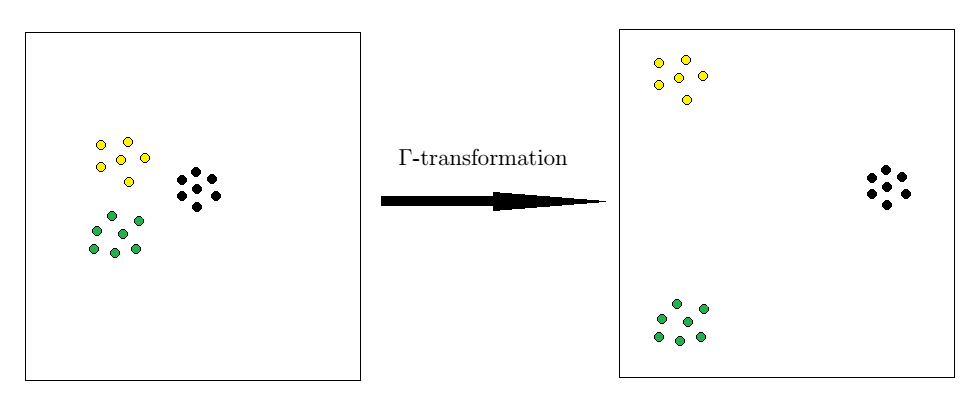
\includegraphics[width=0.75\textwidth]{Paper_figure_1.png}
 \end{center}
 \caption{\textit{This is example of $\Gamma$-transformation for two dimensional data: After the transformation the data points in different clusters are moved away from each other, and the boundary between ``clusters" should be more clear than before.}}
 \label{fig:bsd}
\end{figure}

\begin{figure}[H]
 \begin{center}
   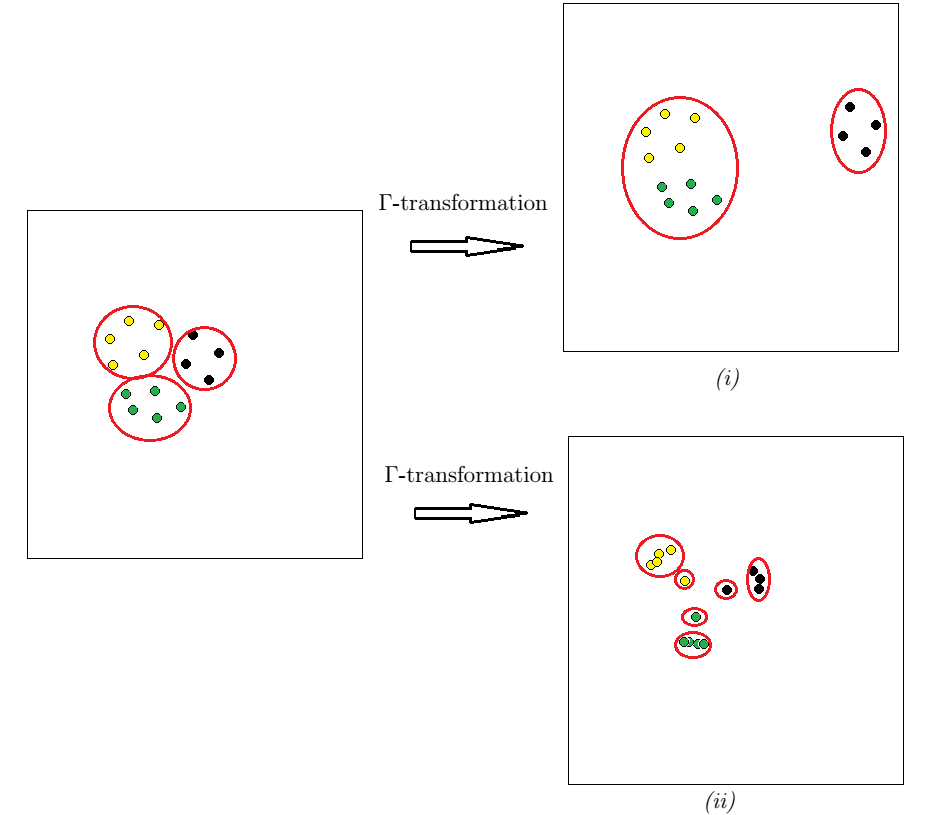
\includegraphics[width=0.65\textwidth]{Paper_figure_2.png}
 \end{center}
 \caption{\textit{This is the example of $\Gamma$-transformation which results in changing the structure of the data: In (i), one of the clusters is pulling away from the other two clusters significantly. In (ii), for each of the cluster, we the shrink all the points together but leave one point out.}}
 \label{fig:bsd}
\end{figure}

Despite this seemingly reasonable assumption that $\Gamma$-transformation always keep the structure of the data the same, actually, in many cases (as \textit{Figure 2} shows), $\Gamma$-transformation will create undesirable transformation, in which the perturbed version of data should be clustered differently. For example, in (i), suppose we move one cluster infinitely away from other clusters, obviously it is a legitimate $\Gamma$-transformation, but the resulting data should be partitioned into  two clusters. However, consistency theorem, if hold, will require the clustering algorithm to produce three clusters as before. Similarly, in (ii), for each cluster, without breaking the constraints of $\Gamma$-transformation, if we shrink all the points together, but leave one points out, it should be more reasonable to partition the data in the way shown in \textit{Figure 2}.

These problems with consistency theorem motivate us to study the property of $\Gamma$-transformation, try to figure out in which case does $\Gamma$-transformation change the structure of the data set.
\section{Investigate the properties of $\Gamma$-transformation by Simulation} \label{sec:framework}
\subsection{Our approach} \label{subsec:approach}
We are taking a numerical approach to investigate how $\Gamma$-transformation change the structure of the data. The general idea is that suppose we have a data set, we first apply some clustering algorithm on this data set, which produce a partition $\Gamma$. Then, we apply $\Gamma$-transformation to this data set for numerous times, and each time we will obtain a different data set. For a clustering algorithm which doesn't satisfy consistency property, if we apply the algorithm to these data sets, it should produce different partition results. We want to figure out what kind of $\Gamma$-transformation will result in partitions which are the same as the partition $\Gamma$ . To decide whether two partition results are the same, we need have some ``measurement", which could measure the difference between two partition, we will discuss various criteria to measure this difference in the third sub-section.

The implementation of these numerical analysis rely on the Python and several libraries including numpy, scikit-learn, etc. We enclose important part of code in Appendix B (The full lists of code can be found on my personal  \href{https://github.com/Zehui127/clusteringResearch2019}{github page}).

\subsection{Generate data points by $\Gamma$-transformation} \label{subsec:blue}
Clustering algorithms can be classified into two groups by the types of required inputs: for algorithms like k-means, we will need the specific coordinates of the every points in the data set, but for algorithm like single-linkage and k-medoids, they only need the distance functions as the input, then they can produce the partition results. To apply a $\Gamma$-transformation on the data set with specific coordinates will be very difficult(actually it is computational impossible on any personal computer even small workspace, when the data set become relatively big\footnote{Recall $\Gamma$-transformation require that we can only decrease the distance between the points within a cluster, and increase the distance between the point in different point. Suppose we have n points in the data set, then when we move one point, we will need to exam $n-1$ equations to make sure our movement satisfy all the inequality. On the other hand, if we are working on the distance matrix, we don't need to worry about these constraints}). So we restrict our scope to the algorithms like single-linkage and k-medoids, which don't need the coordinates. Then in this case, to apply a $\Gamma$-transformation, we simply modify the distance function following the constraints of $\Gamma$-transformation.

With the scope restricted, a dataset containing $N$ data points can be denoted by a $N\times N$ distance matrix $X$, where $X_{i,j}$ refer to the distance between points $i$ and $j$, and it is symmetric matrix with diagonal elements equal to zero. Suppose we have a dataset $X$, a clustering function $f$, and $\Gamma = f(X)$. If we independently apply $\Gamma$-transformation to the dataset for $n$ time, we can obtain a set of distance matrices $D = \{X_1',X_2',\ldots , X_n'\}$, where each element $X_i'$ is the resulting distance matrix from a random $\Gamma$-transformation. Two things need to be noticed: First, every $X_i'$ is produced independently from $X$. Secondly, $\Gamma$-transformation from $X$ to $X_i'$ can make any changes to original distance matrix $X$, it is a completely random process. We enclose the python code of $\Gamma$-transformation in Appendix B, it is a function called \textbf{perturb\_distance\_matrix()}, which take the original distance matrix $X$ and partition $\Gamma$ as the input, and return a distance matrix produced from some random $\Gamma$-transformation.

What is the use of these distances matrices? Well, each of these distance matrices are produced from a ``$\Gamma$-transformation"; Among these transformations, some of the them will change the structure of the original dataset, in which case we expect to see that $f(X_i')\neq \Gamma$, while in the case where the structure of the dataset is preserved, we will expect $f(X_i')= \Gamma$.  Our aim is to target these good $\Gamma$-transformations among $D$, then try to come up with some quantities or models to capture these good $\Gamma$-transformations in the unseen cases. To identify ``good $\Gamma$-transformations", we will apply $f$ to all the elements of distance matrices $D$, which results in a set of new partition $P = \{\Gamma_1',\Gamma_2' \ldots \Gamma_n' \}$, where $\Gamma_i = f(X_i')$. We want to find all $i\in \{1,2\ldots n\}$ such that $\Gamma_i' = \Gamma$, but how can we compare two partitions? We will look at this problem in next section.

\subsection{Measure the difference between partition results} \label{subsubsec:red}
The task here is to compare two partitions of the same dataset, many criteria, such as Jaccard index, Variation of Information distance \cite{meilua2003comparing} and Rand index, can be used to describe the difference between two partitions. All these criteria follow a similar idea: the difference between two clusters is defined in terms of the number of points, or pairs of points two partition disagree \cite{von2010clustering}. In this paper, we will use an variation of a simple criteria - \textbf{Adjusted rand index} , this criteria is based on Rand index, but normalized to have better property. Let's first define Rand index.

Given a dataset of $n$ points $S = \{1,2\ldots n\}$ and two partition of $S$: $\Gamma=\{C_1,C_2\ldots \}$ and $\Gamma' = \{C_1',C_2'\ldots\}$, where $C_1,C_2\ldots$ and $C_1',C_2'\ldots\ $ are non-overlap subsets. 
	\begin{itemize}
\item Let $x =|S^*|$, where $S^*=\{(i,j)|i,j\in C_l$ and $i,j\in C_k' \}$
  
\item Let $y =|S^{**}|$, where $S^{**}=\{(i,j)|i\in C_{l_1},j\in C_{l_2}$ and $i\in C_{k_1}',j\in C_{k_2}' \} $
\end{itemize}
Rand Index, Rd, is defined as:
\begin{equation}
 Rd = \frac{x+y}{{n\choose 2}}
\end{equation}
${n\choose 2}$ is the total number of possible choices of pair. Rand index can be interpreted as the probability that $\Gamma$ and $\Gamma'$ will agree on a randomly chosen pair. The range of Rand index is $[0,1]$, when $Rd(\Gamma,\Gamma') =1$, $\Gamma$ and $\Gamma'$ are exactly the same, while $Rd(\Gamma,\Gamma') =0$ means two partition do not agree on any pair of points. However, Rand index is not often used directly, because it have two obvious drawbacks: For one, in practice, the value of Rand index is ususally in the range between $[0.5,1]$. Also, its baseline value can be high and does not take a constant value \cite{vinh2010information}. 

Due to these reasons, \textbf{Adjusted rand index} is introduced, it is proposed in 1985\cite{hubert1985comparing}. Adjusted rand index basically is a normalized version of Rand index, it is given by following formula:
\begin{equation}
 \textrm{Adjusted Rand Index} =  \frac{\textrm{Rand Index}-\textrm{Expected Rand Index}}{\textrm{Maximum Rand Index}-\textrm{Expected Rand Index}}
\end{equation}
Expected Rand Index is calculated by assuming the generalized hypergeometric distribution of randomness, we will not go into the details of this distribution. But after this normalization operation, Adjusted Rand index will be a better measurement for the difference between two clusters, it is bounded above by 1 and only equals to 1 if two partition are exactly the same, and close to zero when we randomly label the data into clusters. Furthermore, in practice, the value of the Adjusted Rand Index will be evenly ranging from 0 to 1.

In the simulation, we write our Rand Index function, but make use of the \textbf{Adjusted\_rand\_index()} function in sklearn library for efficiency purpose. Here is the graph showing the property of rand index and adjusted rand index.

\begin{figure}[H]
 \begin{center}
   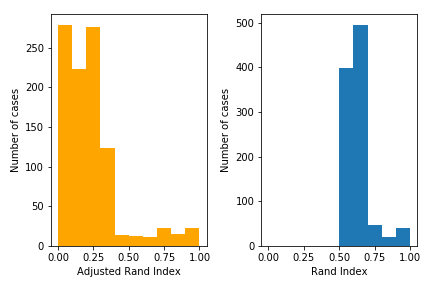
\includegraphics[width=0.4\textwidth]{adjusted.png}
 \end{center}
 \caption{\textit{We randomly generate 1000 pairs of partitions, then compute the Adjusted Rand Index and Rand Index for these pairs. It can be clearly seen that the value of Adjusted Rand Index is distributed across $[0,1]$, while Rand Index without Normalization concentrate on $[0.5,1]$}}
 \label{fig:bsd}
\end{figure}


\section{Simulation Results} \label{sec:red}
Following the framework proposed in section \ref{subsec:blue}, below is the simulation we did for investigating the property of $\Gamma$-transformation: We start from the original dataset, represented by distance matrix $X$, then let $\Gamma = f(X)$, where $f$ is the selected clustering algorithm we want to study. Apply $\Gamma$-transformation on $X$ for multiple times to get the perturbed version of dataset $D = \{X_1',X_2'\ldots X_n'\}$. Applying $f$ to every element of $D$ will result in a set of partitions $P = \{f(X_1'),f(X_2')\ldots f(X_n')\}=\{\Gamma_1',\Gamma_2' \ldots \Gamma_n' \}$. Finally, we calculate corresponding Adjusted Rand Index(ARI) for each of these partitions $\{ARI(\Gamma_1',\Gamma),ARI(\Gamma_2',\Gamma)\ldots ARI(\Gamma_n',\Gamma)\}$. \textit{Table-1} present the psudo-code for the simulation steps.
\subsection{Simulation for K-mediods} \label{subsec: kmediods}


In the first experiment, $f$ is set to be \textbf{k-mediods}. We try $n=1000$, $n=10000$ and $20000$, \textit{Figure-4} shows the raw frequency of the Adjusted Rand Index in these cases, together with the Adjusted Rand Index under random perturbed data. Compared with the distribution of ARI upon random perturbed data which is the \textit{Figure-4}(a), the distribution of the ARI upon $\Gamma$-transformation clearly shows that $\Gamma$-transformation has the tendency to preserve the structure of the data. Even more remarkable, as $n \rightarrow \infty$, ARI tend to have a fixed \textbf{Probability Density Function}. In \textit{Figure-5}, We draw the density plot of the ARI when $n=10000,20000\ldots 70000$ (the density is estimated by the sum of multiple Gaussian distribution), and it shows that the density function tends to converge to the same function.
\begin{figure}[H]
 \begin{center}
   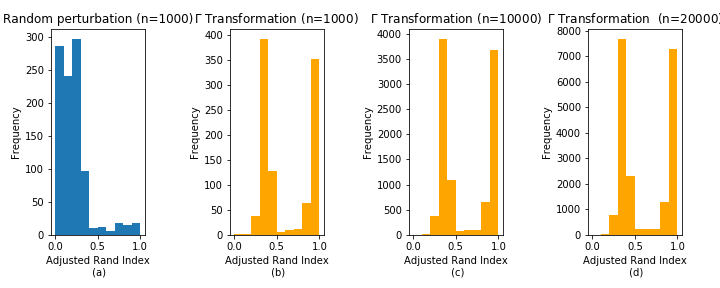
\includegraphics[width=0.7\textwidth]{simulate1.png}
 \end{center}
 \caption{\textit{Histogram of Adjusted Rand Index(ARI) for K-mediods. $n$ distance matrices $\{X_1',X_2'\ldots X_n'\}$ are created from $X_{origin}$ by $\Gamma$-transformation, $Y$ are created from random perturbation. (b),(c)and (d) shows histogram of $ARI(f(X_j'),f(X_{origin}))$ when $n=1000,10000,20000$ respectively.
(a) shows the histogram of $ARI(f(Y),f(X_{origin}))$ when $n =1000$.}}
 \label{fig:bsd}
\end{figure}

\begin{figure}[H]
 \begin{center}
   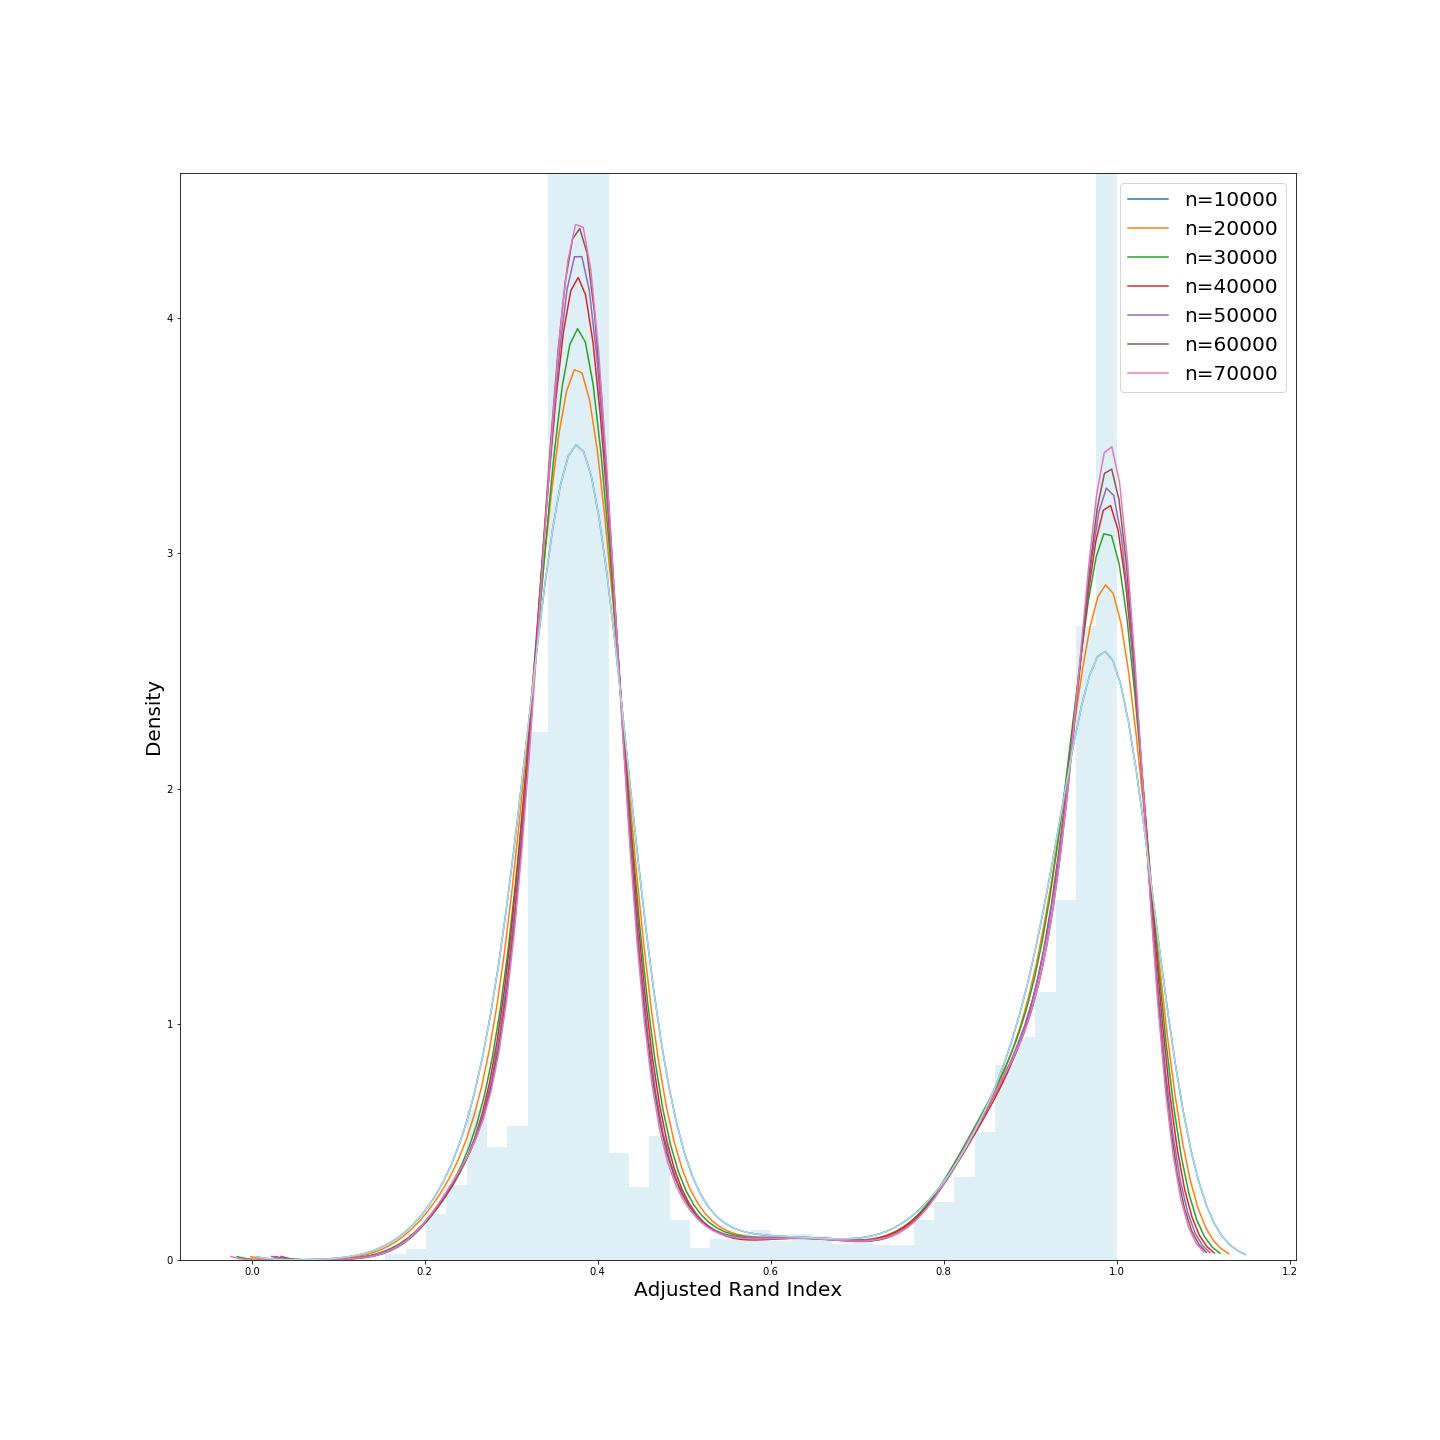
\includegraphics[width=0.7\textwidth]{simulate2.png}
 \end{center}
 \caption{\textit{We estimate the density function of $ARI(f(X_j'),f(X_{origin}))$ by the summing up Gaussian Distribution, this graph shows that as we increase the number of distance matrices, the density function converge to a ``true" density function.}}
 \label{fig:bsd}
\end{figure}

\subsection{Simulation for Complete Linkage} \label{subsec: Complete-linkage}
Complete-linkage is similar to Single-linkage Algorithm we discuss in the section \ref{subsec:Single-linkage}, it also take a bottom up approach - start from regarding each data points as a cluster, then merge two clusters with least dissimilarity\cite{christopher2008introduction}. But the dissimilarity is defined in following manner.
\begin{definition}
Let G,H represent two clusters, d is the distance function of the data set, then dissimilar $d_{SL}$ is defined as:
$d_{SL}(G,H) = \max_{i\in G,i'\in H}d_{ii'} $
\end{definition}
Here we let $f$ be Complete-linkage with k-clusters termination condition, and go through the same procedure as we did in previous section. \textit{Figure-\ref{fig:single-linkage}} shows the histogram of the ARI when $n=1000$ and $4000$. Compared to the histogram of K-mediods, it has heavier tail at $ARI = 1$, which could be interpreted as an evidence for that Complete-linkage are ``more consistency".  We also try to estimate the probability density function of ARI, but this time, instead of using mixture Gaussian Distribution, we assume the density function has a Gamma-distribution, then use the data to estimate the parameter of it. \ref{fig:single-linkage2} shows the estimated graph.

\begin{figure}[H]
 \begin{center}
   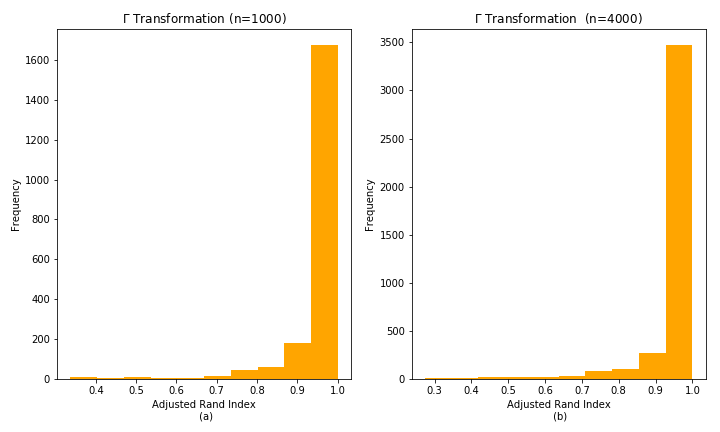
\includegraphics[width=0.7\textwidth]{simulate2_1.png}
 \end{center}
 \caption{\textit{Histogram of Adjusted Rand Index(ARI) for complete-linkage when $n=1000$ and $4000$ }}
 \label{fig:single-linkage}
\end{figure}

\begin{figure}[H]
 \begin{center}
   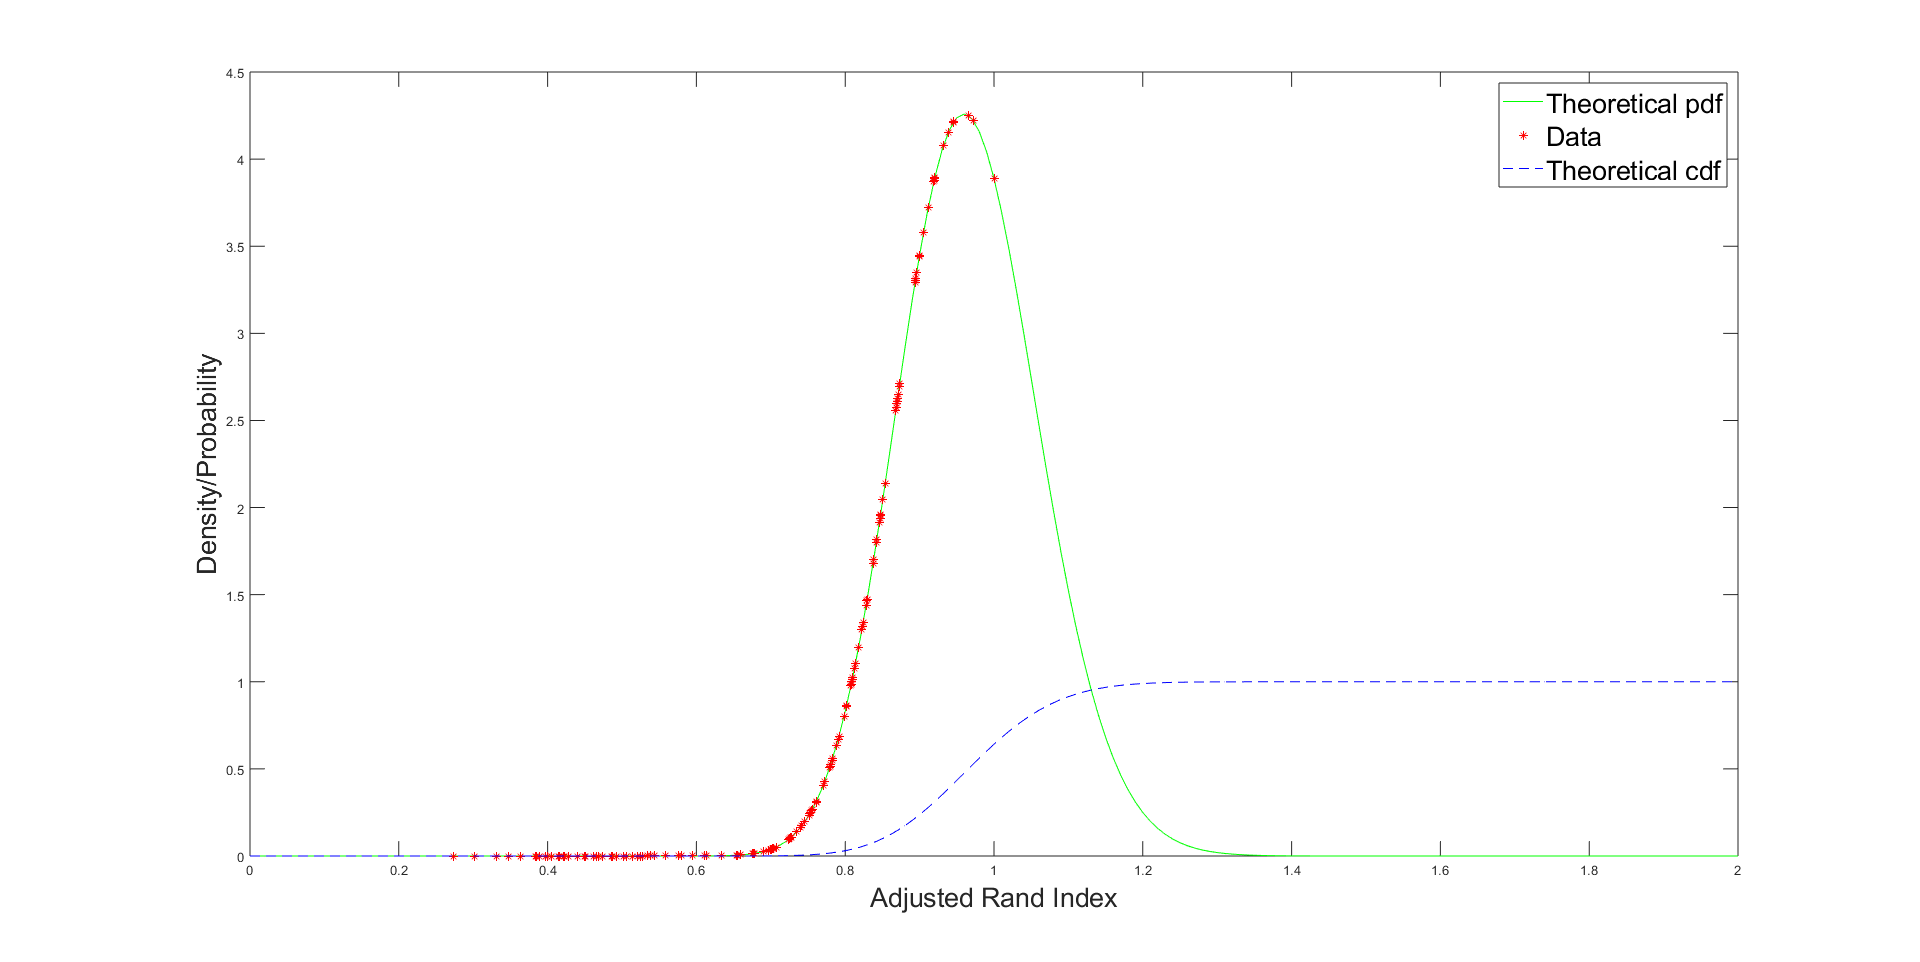
\includegraphics[width=1\textwidth]{Complete-linkage-cdf.png}
 \end{center}
 \caption{\textit{Estimated density function and cumulated density function of $ARI$ for Complete linkage}}
 \label{fig:single-linkage2}
\end{figure}

\subsection{Implication and limitation of the simulation} \label{subsec: simulationSum}
There are two important observations we get from the simulation process. The first one is that Adjusted Rand Index(ARI) after $\Gamma$-transformation had a very heavy tail at $ARI=1$, which is consistent with our intuition for $\Gamma$-transformation - it shouldn't change the structure of data set. The second observation is that different clustering algorithms will have different ARI distribution, for K-mediods, it has two 	``peaks" at ARI = 1 and ARI = 0.4, while for Complete-linkage, distribution of ARI can be fitted relative good by Gamma distribution. 

For Complete-linkage and K-mediods, $\Gamma$ transformation lead to a skewed distribution of ARI (The relative frequency of $ARI =1$ is higher than other value). Although we haven't tried all the clustering algorithm, it is reasonable to make the assumption that there are many other clustering algorithms satisfying this skewed distributed feature. So we formalize our assumption and state it as a refined version of consistency property, calling it \textbf{$\beta$-Partial Consistency}. 
Given $0<=\beta<=1$, it is defined as following:
\begin{definition}
$\beta $-Partial Consistency. Clustering algorithm $f$ satisfy $\beta$-Partial Consistency $\iff$ Given $D=\{d_1',d_2'\ldots d_n'\}$ contains $n$ $\Gamma$-transformation of distance function $d$, as $n\rightarrow \infty$, there exists at least $\beta *n$ number of $d_i'\in D$ satisfying $f(d_i')=f(d)$ 
\end{definition}
Recall the original consistency property, it is actually a special case of $\beta $-Partial Consistency when $\beta = 1$. The original consistency property is a very strict one, only a small portion of clustering algorithm satisfy this property, but a wider range of clustering algorithms could satisfy $\beta$-Partial Consistency. From the simulation, we can see the potential existence of this property for \textbf{K-mediods} and \textbf{Complete-Linkage}. Figure-\ref{fig:single-linkage4} shows that the relative frequency of $ARI=1$ could tend to a fixed value as we increase the value of $n$.

\begin{figure}[H]
 \begin{center}
   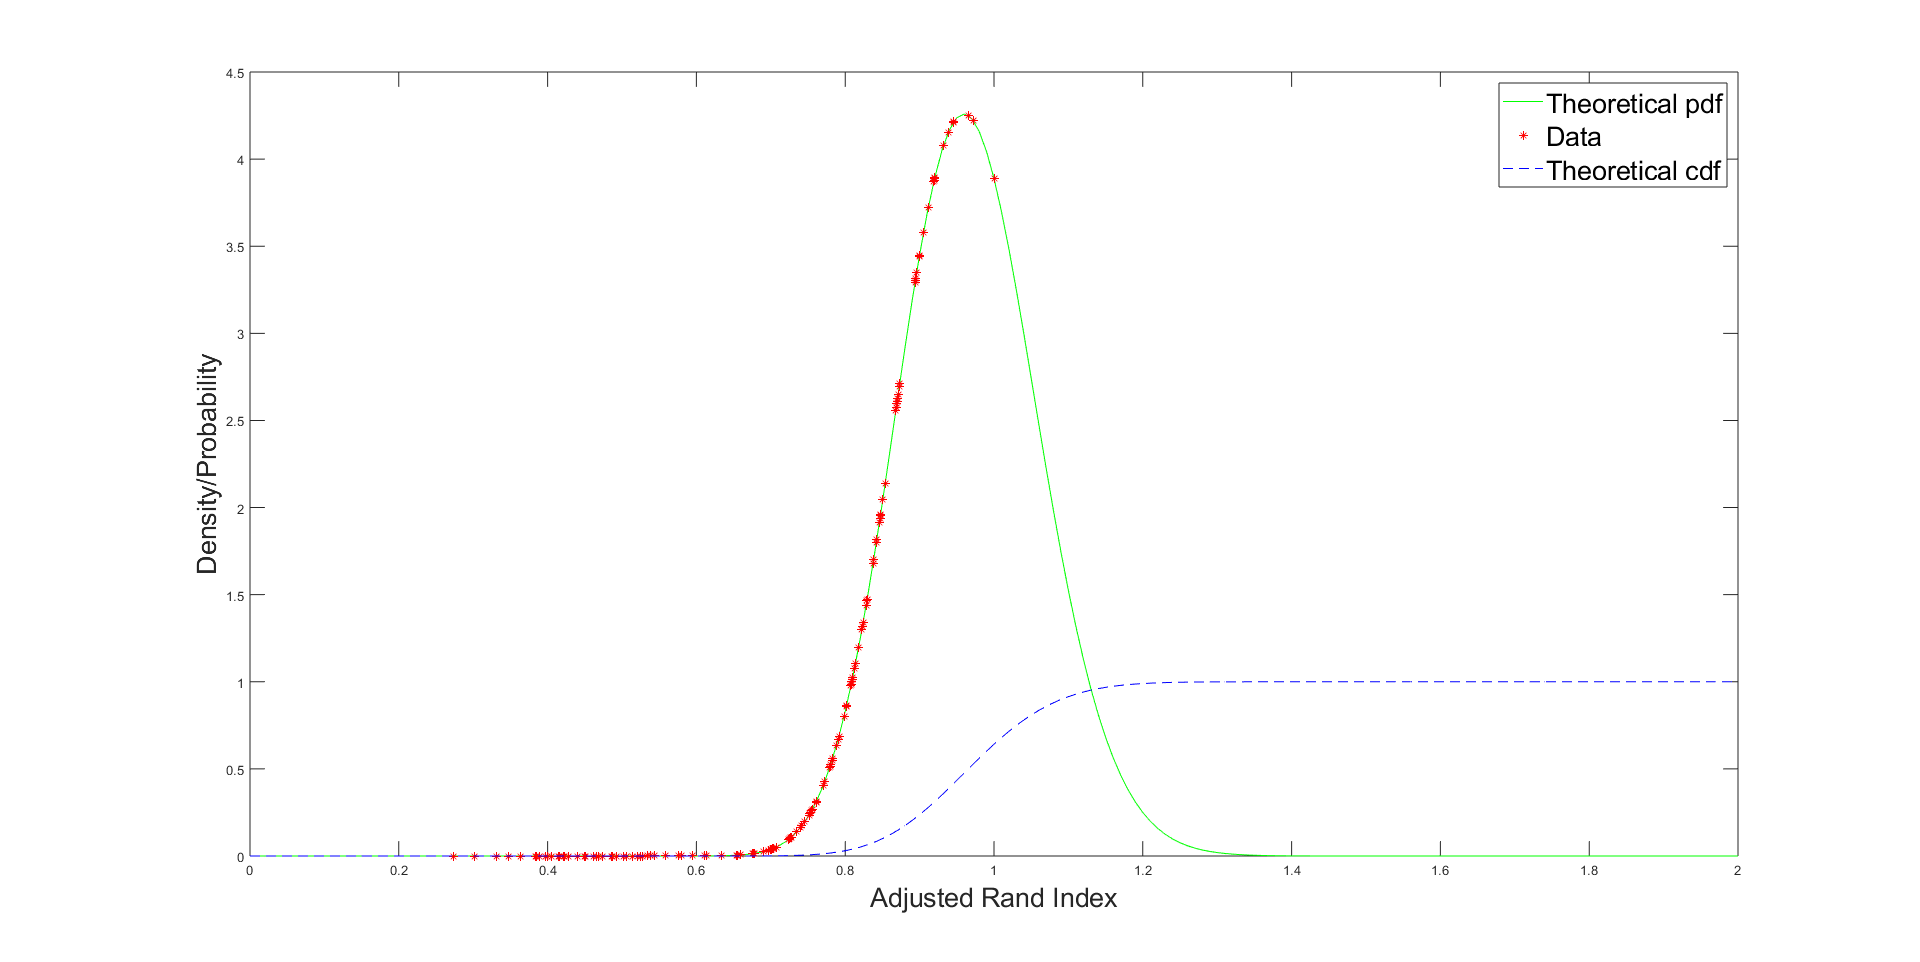
\includegraphics[width=1\textwidth]{Complete-linkage-cdf.png}
 \end{center}
 \caption{\textit{Change of the relative frequency of ARI = 1:Y-axis shows \textbf{relative frequency of} $1$ = $\frac{\textsl{Frequency of ARI}=1}{\textsl{Total number of cases}} $ for Complete-linkage algorithm, x-axis shows the value of n. As n increase, this value tend to a fixed value=0.78.}}
 \label{fig:single-linkage4}
\end{figure}

This simulation process has several limitations: First of all, we only work on two of the clustering algorithms, so the simulation results could differ for other clustering algorithm. Secondly, we haven't proved that these two algorithms satisfy \textbf{Partial Consistency}, currently, it is only an assumption from simulation results, and mean to provide a direction for future study. Thirdly, our python implementation of $\Gamma$-transformation can only deal with distance matrix but not specific coordinates due to the limitation of computational resources.

\section{Simulation results: Classification with SVM and other methods} \label{sec:Classification}










\section{Conclusions} \label{sec:conclusions}



\newpage

\appendix

\section{Remaining Proof for Single-linkage} \label{app:proof}
In this appendix, we provide the proof for \textit{Theorem \ref{second theorem}} and  \textit{Theorem \ref{third theorem}}.
\begin{proof}
\textit{theorem \ref{second theorem}}

\noindent Given data set $S$ and distance function $d$, and $f$ be the single-linkage with k-clusters termination condition. 

Scale-Invariance of $f$ is easy to prove, suppose 
\end{proof}

\section{ Pyhton code } \label{app:calculations}

In this appendix we verify equation \eqref{eq:myeq1}.

\newpage

\bibliographystyle{unsrt}
\bibliography{References}

\end{document}
